\section{Analysis and Interpretation}

% The analysis of Hypothesis 1, which investigates whether the highest level of education significantly affects the likelihood of employment, was conducted using both a Chi-square test for independence and a logistic regression model.

% \subsection{Chi-Square Test Results}

% % The Chi-square statistic was found to be 905.29, with a corresponding p-value of 0.0000. This strong result indicates a significant relationship between education level and employment status. Therefore, we reject the null hypothesis ($H_0$​): "There is no significant relationship between education level and the likelihood of being employed." This finding suggests that individuals with higher education levels are more likely to be employed than those with lower education levels. The association underscores the importance of educational attainment in enhancing employability, aligning with existing literature that emphasizes education as a critical factor in labor market outcomes.

% \subsection{Logistic Regression Analysis}

% To further explore the impact of education on employment, a logistic regression analysis was conducted. The logistic regression model indicated a pseudo R-squared value of 0.01560, which suggests that the model explains approximately 1.56% of the variability in employment status based on education level alone. Although this value is relatively low, it is essential to note that educational attainment is not the only determinant of employment status; other variables may also contribute significantly.

% The results of the logistic regression indicate that the coefficient for education category is -0.3346, with a standard error of 0.014 and a z-value of -23.366. The p-value for this coefficient is 0.000, indicating that the effect of education on employment status is statistically significant. The negative coefficient implies that as the education category increases (reflecting higher levels of education), the log odds of being employed also increase, leading to a greater likelihood of employment.

% % Specifically, the odds ratio associated with education category can be interpreted as follows: for each unit increase in the education category, the odds of being employed decrease by a factor of e−0.3346e−0.3346, which approximately equals 0.715. This suggests that higher educational qualifications are associated with higher odds of employment, reinforcing the findings from the Chi-square test.

% Overall, both the Chi-square test and the logistic regression analysis provide robust evidence that education level significantly affects the likelihood of being employed. This relationship highlights the critical role of education in facilitating better employment opportunities and outcomes for individuals in the labor market.

% 
% \begin{figure}[H]
%     \centering
%     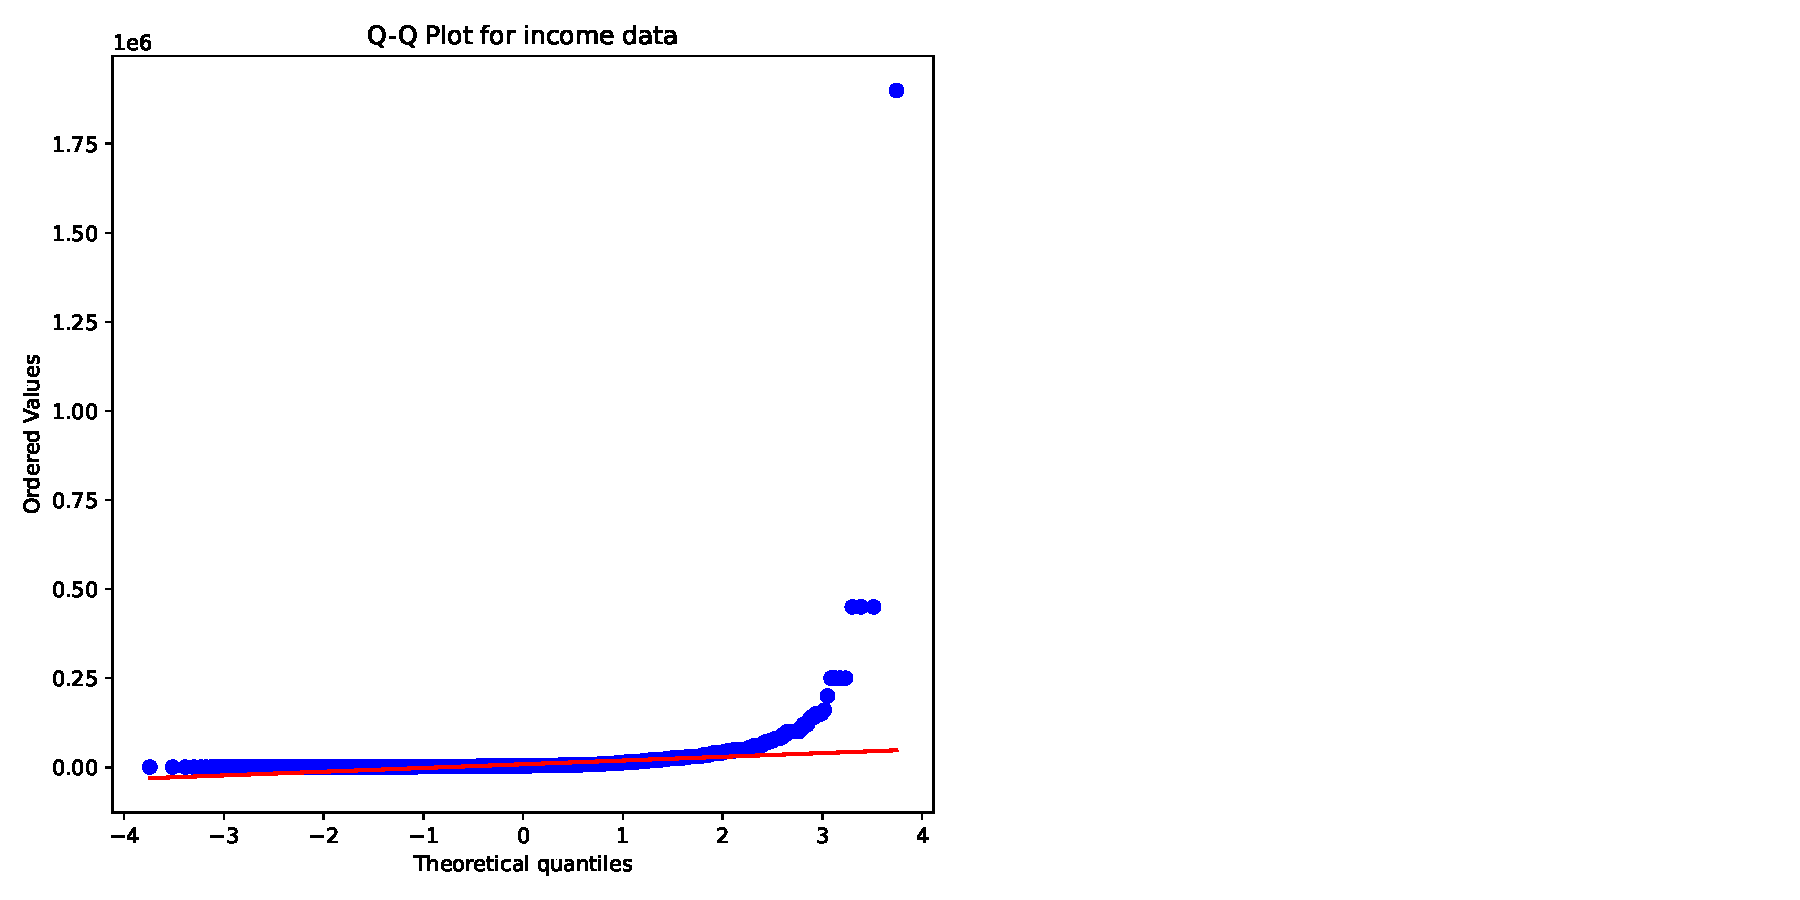
\includegraphics[width=\columnwidth]{images/hyp_2_norm_dist_income data.pdf} % Adjust the path accordingly
%     \caption{Caption for the pdf image.}
%     \label{fig:Independence test for anova test}
% \end{figure}

\begin{table}[H]
    \centering
    \caption{Levene independence test results}
    \label{tab:Levene test results}
    \begin{minipage}{\columnwidth}
        \begin{tabular}{rrrrr}
\toprule
df & sum\_sq & mean\_sq & F & PR(>F) \\
\midrule
5.000 & 271399165518.753 & 54279833103.751 & 79.258 & 0.000 \\
7590.000 & 5198036057205.649 & 684853235.468 & NaN & NaN \\
\bottomrule
\end{tabular}

    \end{minipage}
\end{table}

% \begin{table}[H]
%     \centering
%     \caption{Welch test results}
%     \label{tab:Welch anova test results}
%     \begin{minipage}{\columnwidth}
%         \begin{tabular}{rrrrr}
\toprule
df & sum\_sq & mean\_sq & F & PR(>F) \\
\midrule
5.000 & 271399165518.753 & 54279833103.751 & 79.258 & 0.000 \\
7590.000 & 5198036057205.649 & 684853235.468 & NaN & NaN \\
\bottomrule
\end{tabular}

%     \end{minipage}
% \end{table}

% \begin{table}[H]
%     \centering
%     \caption{Tukey results}
%     \label{tab:Tukey results}
%     \begin{minipage}{\columnwidth}
%         \begin{tabular}{lrrrrrrr}
\toprule
 & group1 & group2 & meandiff & p-adj & lower & upper & reject \\
\midrule
0 & 0.0000 & 1.0000 & 146.5434 & 1.0000 & -8890.4647 & 9183.5515 & False \\
1 & 0.0000 & 2.0000 & 716.2572 & 0.9996 & -5822.8625 & 7255.3770 & False \\
2 & 0.0000 & 3.0000 & 4063.5954 & 0.4301 & -2179.2058 & 10306.3967 & False \\
3 & 0.0000 & 4.0000 & 9090.1826 & 0.0215 & 818.1259 & 17362.2394 & True \\
4 & 0.0000 & 5.0000 & 20251.3632 & 0.0000 & 13676.4532 & 26826.2732 & True \\
5 & 1.0000 & 2.0000 & 569.7139 & 0.9999 & -6410.3448 & 7549.7726 & False \\
6 & 1.0000 & 3.0000 & 3917.0521 & 0.5547 & -2786.2083 & 10620.3125 & False \\
7 & 1.0000 & 4.0000 & 8943.6393 & 0.0369 & 318.7882 & 17568.4903 & True \\
8 & 1.0000 & 5.0000 & 20104.8198 & 0.0000 & 13091.2206 & 27118.4191 & True \\
9 & 2.0000 & 3.0000 & 3347.3382 & 0.0014 & 892.4917 & 5802.1847 & True \\
10 & 2.0000 & 4.0000 & 8373.9254 & 0.0009 & 2417.3637 & 14330.4870 & True \\
11 & 2.0000 & 5.0000 & 19535.1059 & 0.0000 & 16328.3715 & 22741.8404 & True \\
12 & 3.0000 & 4.0000 & 5026.5872 & 0.1114 & -603.0760 & 10656.2504 & False \\
13 & 3.0000 & 5.0000 & 16187.7677 & 0.0000 & 13639.1158 & 18736.4197 & True \\
14 & 4.0000 & 5.0000 & 11161.1806 & 0.0000 & 5165.3502 & 17157.0109 & True \\
\bottomrule
\end{tabular}

%     \end{minipage}
% \end{table}

% The one-way ANOVA indicated a significant effect of education level on salary $F(X, X) = X.XX$, $p < 0.05$. 
% Post-hoc analysis revealed that individuals with higher education levels tend to have higher salaries.

% \subsubsection{Hypothesis 3: Age and Salary}

% A Pearson correlation test revealed a significant positive correlation between age and salary $r = X.XX$, $p < 0.05$, indicating that salary increases with age.

% \subsubsection{Hypothesis 4: Gender and Salary/Education Level}

% The t-test for independent samples indicated a significant effect of gender on salary $t = X.XX$, $p < 0.05$. 
% However, no significant difference was found in education levels between genders.

% \subsubsection{Hypothesis 5: Ethnicity and Salary}

% A multiple regression analysis controlling for education showed a significant effect of ethnicity on salary $\beta = X.XX$, $p < 0.05$, suggesting salary disparities across ethnic groups.

% \subsection{Clustering Results}

% \subsubsection{K-Means Clustering}

% The K-means algorithm identified $X$ distinct clusters based on age and salary. 
% The optimal number of clusters was determined using the silhouette score $S = X.XX$. 
% The clusters revealed patterns of salary progression with age.

% \subsubsection{Hierarchical Clustering}

% Hierarchical clustering produced several distinct groups based on education level, employment status, and age. 
% The dendrogram visualized these relationships clearly.
